\section{溶液物性および圧力場の確認}
\subsection{粘度計測}
球落下実験を行う試験溶液として,異なる質量濃度のPAA溶液を製作した.この製作した溶液の粘度特性を得るため,粘度計を用いて計測を行った.なお,溶媒中の溶質が不均一な状態や,混合時に混入する気泡が存在する状態では,溶液の粘度が正しく計測できない.十分な溶質拡散や脱泡のために時間を要するため,粘度計測は溶液作製直後ではなく,1週間後に行った.それぞれの試料に対し,円錐回転子の回転数を変化させることでせん断速度を変化させ,粘度を各5回計測を行いその平均を求めた.

水道水の粘度計測結果をFig.\ref{fig:water-vis}に示す.なお,縦軸は粘度,横軸はせん断速度を表す.第2.2節においても示したが,コーンロータの回転速度に応じて,液体のせん断速度を変化させた.その結果,粘度は約1.1[mPa$\cdot$ s]でほぼ一定となっていた.これは,水がニュートン流体であり,粘度を比例係数とした速度勾配とせん断応力の比例関係となっているためであると考えられる.

水道水の場合と同様にPAA溶液の粘度計測を行った結果をFig.\ref{fig:PAA-vis}に示す.なお,縦軸は粘度の対数,横軸はせん断速度の対数を表す.ここで,粘度$\mu$はせん断速度$\dot{\gamma}$に対して,粘度定数 k[Pa$\cdot$ $\text{s}^n$],指数$n$を用い Power-law modelに従うものとすると,
\begin{eqnarray}
	\label{eq:power-low}
	\mu=k\cdot\dot{\gamma}^{n-1}
\end{eqnarray}
といった式で与えられる\cite{ref:1}.式(\ref{eq:power-low})を用いて近似線計算を行った結果を,Table \ref{table:power-law}に示す.溶液の濃度が濃いほど,擬塑性を示す$n$は小さくなり,より擬塑性が強くなった.粘性を表す$k$は,濃度の上昇に伴い大きくなった.これらより,濃度が濃くなると,より擬塑性が強く,粘性が大きい流体となったことが分かった.

% //TODO:水の粘度計測結果,要修正?
\begin{figure}[ht]
	\centering
	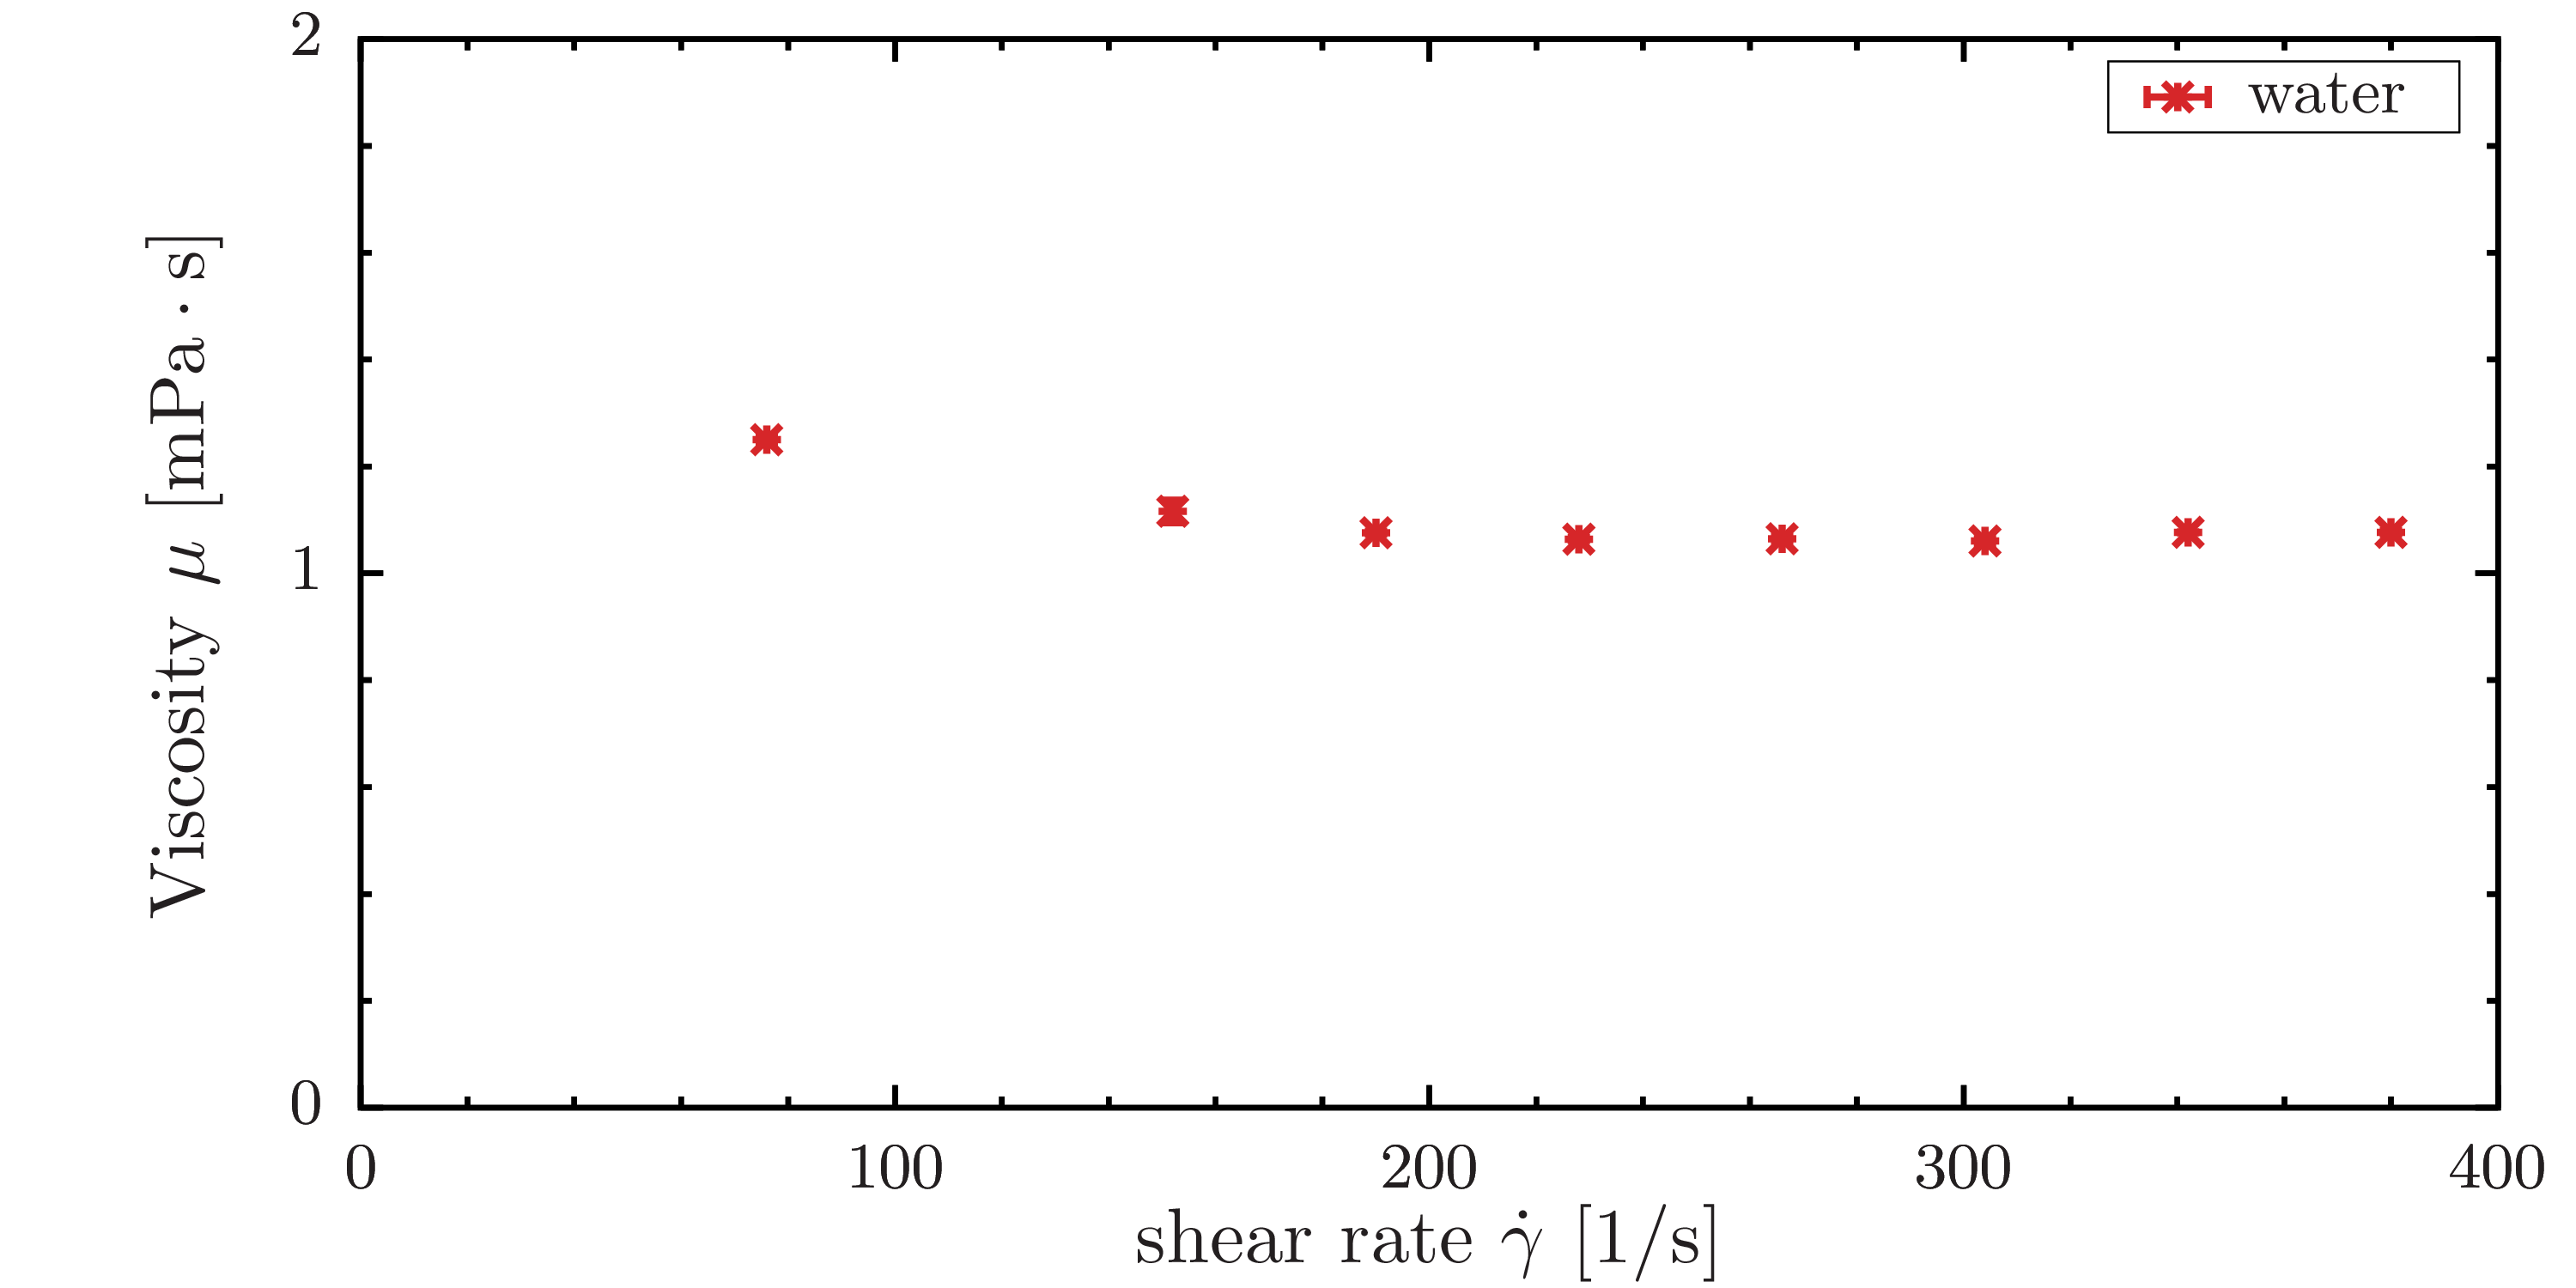
\includegraphics[width=12cm,clip]{4-Results/water.png}
	\caption{Meansured viscosity versus shear rate for tap water.}
	\label{fig:water-vis}
\end{figure}

\begin{figure}[ht]
	\centering
	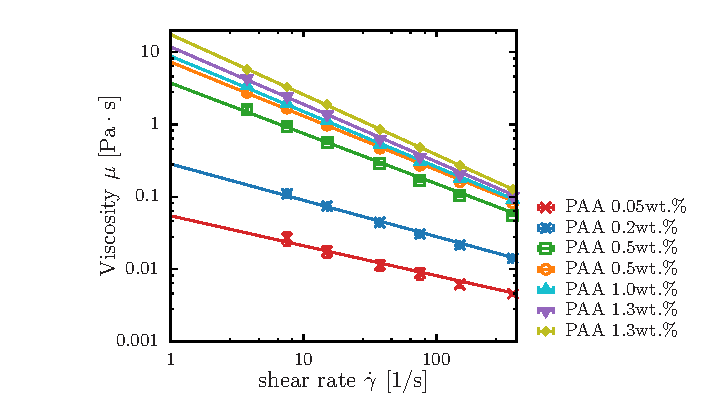
\includegraphics[width=13cm,clip]{4-Results/viscosity.eps}
	\caption{Flow curve for PAA solution.}
	\label{fig:PAA-vis}
\end{figure}

\begin{table}[h]
	\centering
	\caption{Parameters $k$ and $n$ in the power-law model for each experimental result.}
	\label{table:power-law}
	\begin{tabular}{c|c|c|c|c|c|c|c} \hline
		PAA[wt.\%] & 0.05  & 0.2  & 0.5  & 0.7  & 1.0  & 1.3  & 1.5  \\ \hline \hline
		$k$        & 0.054 & 0.28 & 3.7  & 7.3  & 8.8  & 12   & 18   \\
		$n$        & 0.59  & 0.50 & 0.30 & 0.25 & 0.23 & 0.21 & 0.17 \\ \hline
	\end{tabular}
\end{table}

\newpage

% //TODO:圧力振幅の溶液依存性を示す
\subsection{圧力振幅 計測結果}

それぞれの質量濃度において,超音波圧力振幅の計測を行った.超音波圧力振幅の結果をFig.\ref{fig:pressure}に示す.縦軸は水槽底面からの高さ,横軸は圧力振幅である.この結果を元にTable \ref{table:press}に,圧力振幅$\delta{}P$の$y$方向平均値を示す.水槽全体に圧力振幅が発生していることが確認された.

% //TODO:圧力振幅の結果を入れる
\begin{table}[h]
	\centering
	\caption{Averaged value of pressure amplitude.}
	\label{table:press-A}
	\begin{tabular}{c|c|c|c|c|c|c|c} \hline
		PAA[wt.\%]             & 0.05 & 0.2 & 0.5 & 0.7 & 1.0 & 1.3 & 1.5 \\ \hline \hline
		$\bar{\Delta{}P}$[kPa] &      &     &     &     &     &     &     \\ \hline
	\end{tabular}
\end{table}

\begin{figure}[ht]
	\centering
	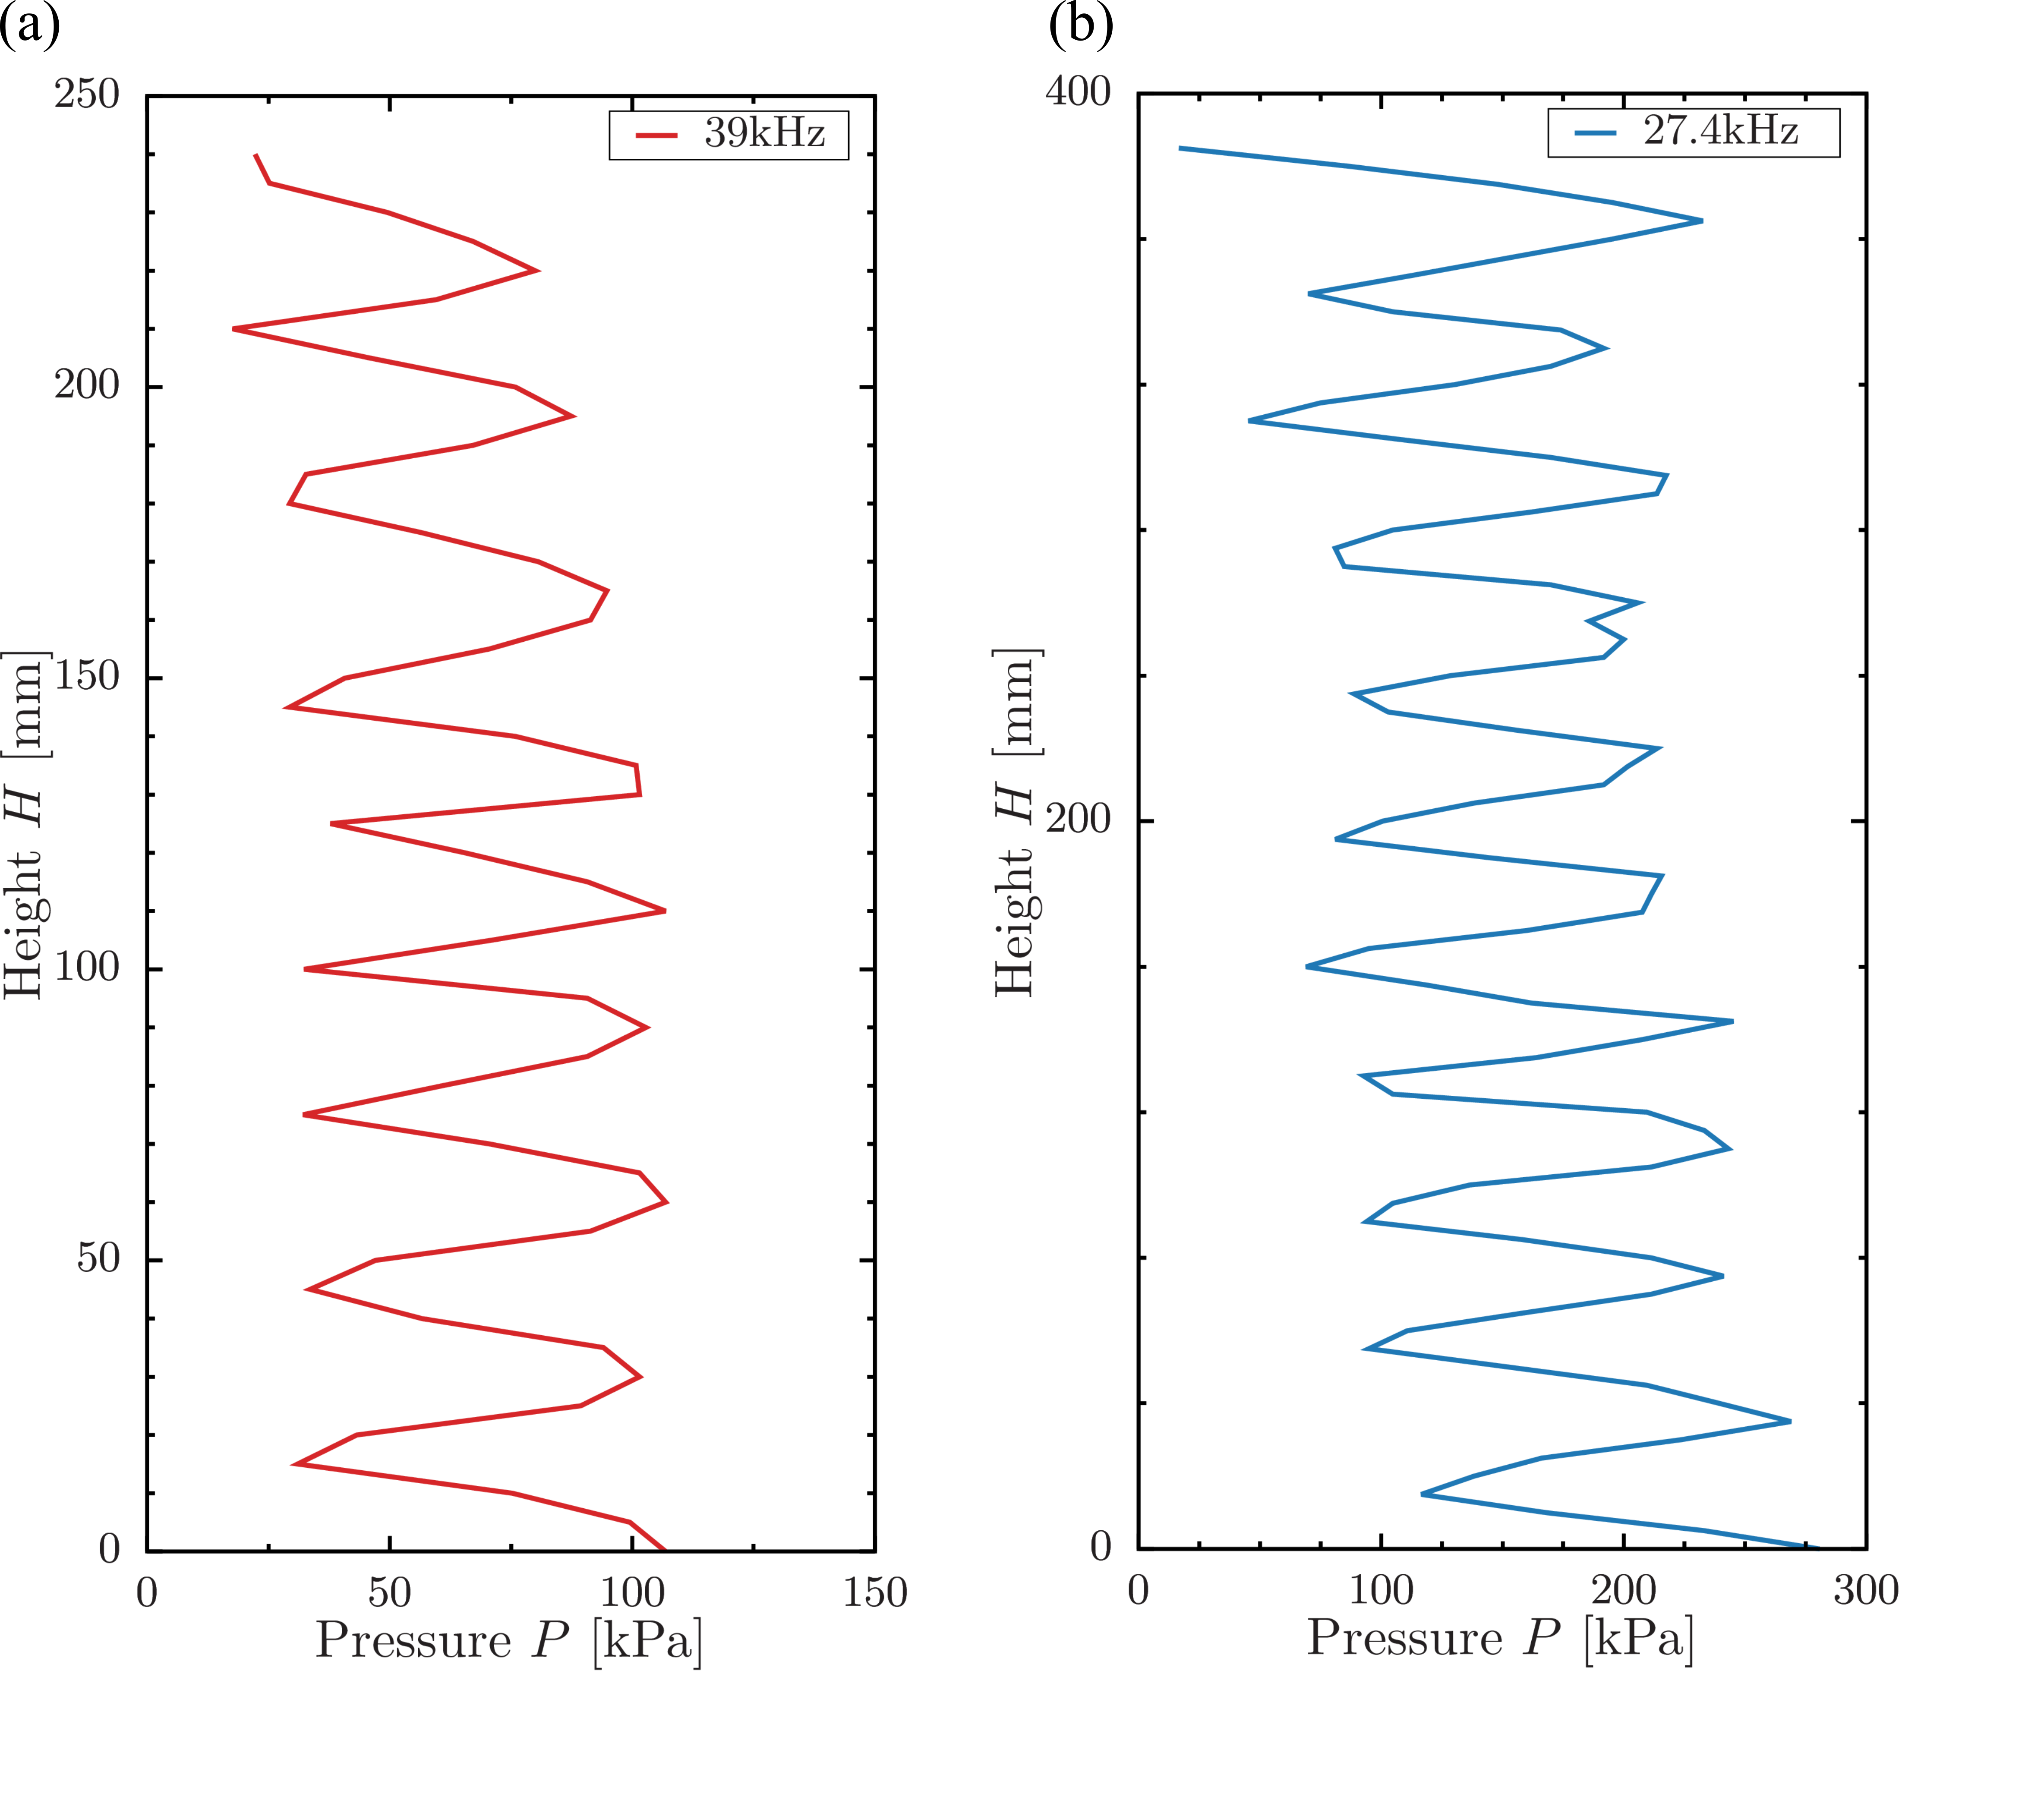
\includegraphics[width=12cm,clip]{4-Results/press.png}
	\caption{Average pressure amplitude in PAA solution.}
	\label{fig:pressure}
\end{figure}
